\documentclass[12pt]{article}
\usepackage{amsmath}
\usepackage{graphicx}
\usepackage{pdfpages}
\usepackage{amssymb}
\usepackage{float}

\title{Extra Credit Assignment}
\author{Ryan C. Bleile}

\begin{document}
\maketitle
\newpage

\section*{Discritizing T}

In order to discritize T, I began with the definition of the left sided Riemann sum to approximate an integral.\\

$$ Sum = \Delta x ( f(a) + f(a + \Delta x) + f(a + 2 \Delta x) + .. f(a + (n-1) \Delta x)) $$

From this we know what we want is:\\

\[ \textbf{A} \vec{f} = \vec{g} \]

Which means that for an interval on a finite range 0 to x:\\

\[ \textbf{A} f(x) = g(x) \]

for a given x. Using this we see that we must preform a partial Riemann sum of the points over this range to make every Af(x) map to a g(x). This gives us a set of equations:

\begin{eqnarray*}
 \Delta x f(0)&=& g(0)\\
 \Delta x (f(0) + f(\Delta x)) &=& g(\Delta x)\\
 \Delta x (f(0) + f(\Delta x) + f(2 \Delta x)) &=& g(2 \Delta x)\\
 \Delta x (f(0) + f(\Delta x) + f(2 \Delta x) + f(3 \Delta x)) &=& g(3 \Delta x)\\
 ... &=& g(n);
\end{eqnarray*} 

In order to produce this list of partial sums which reproduce the full Riemann sum for the full range we can write this as a matrix vector multiplication such that:

\[
\begin{bmatrix}
\Delta x & 0 & 0 & 0\\
\Delta x & \Delta x & 0 & 0\\
\Delta x & \Delta x & \Delta x & 0\\
\Delta x & \Delta x & \Delta x & \Delta x
\end{bmatrix}
\begin{bmatrix}
f(0)\\
f(\Delta x)\\
f(2 \Delta x)\\
f(3 \Delta x)
\end{bmatrix}
=
\begin{bmatrix}
g(0)\\
g(\Delta x)\\
g(2 \Delta x)\\
g(3 \Delta x)
\end{bmatrix}\]

This discritizes T to be:

\[
A =
\Delta x
\begin{bmatrix}
1 & 0 & 0 & 0\\
1 & 1 & 0 & 0\\
1 & 1 & 1 & 0\\
1 & 1 & 1 & 1
\end{bmatrix}
\]

for n = 4.

\section*{Mat Lab Plots}
\begin{center}

\begin{figure}[H]
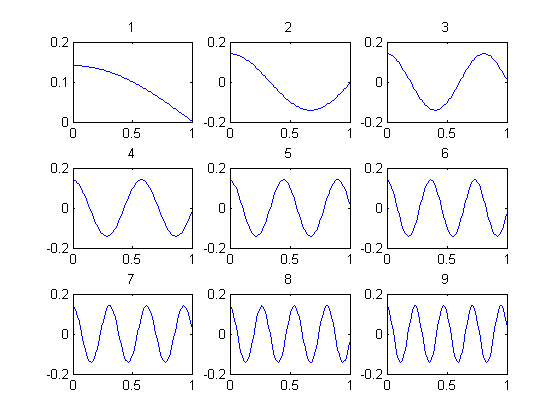
\includegraphics[scale=1]{plot1.png}
\caption{Plot 1: The first 9 eigenvectors in descending order}
\end{figure}

\begin{figure}[H]
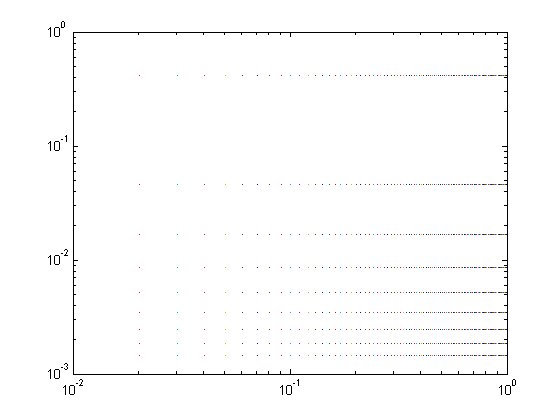
\includegraphics[scale=1]{plot2.png}
\caption{Plot 2: Log scale eigenvalues. It appears that the eigenvalues are converging to zero in the same manner as a dying exponential, like a decaying function. After looking closely at different numbers of plotted eigen vectors i have noticed that after about nine or ten eigen vectors the rest are so close together that there is very little difference. Also the values are very small and there fore more susceptible to small amounts of noise. It appears that we could approximate our f with far fewer eigenvectors than N. And hence 10 eigenvectors which make the biggest difference could be used to approximate f in equation 2. Later we do this approximation for 9.}
\end{figure}

\begin{figure}[H]
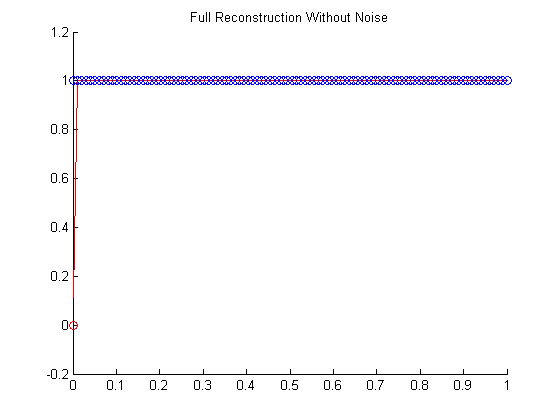
\includegraphics[scale=1]{plot3.png}
\caption{Plot 3: A full reconstruction of f using g = x with no noise}
\end{figure}

\begin{figure}[H]
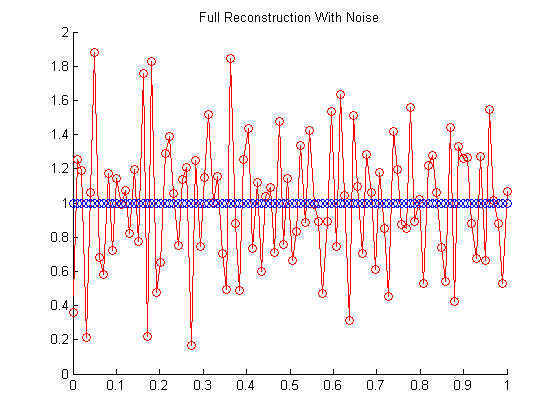
\includegraphics[scale=1]{plot4.png}
\caption{Plot 4: A full reconstruction of f using g = x with noise}
\end{figure}

\begin{figure}[H]
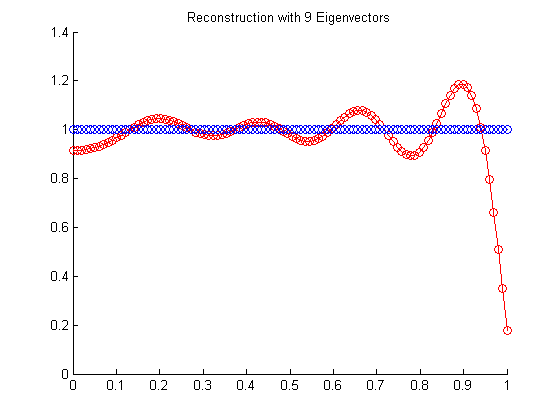
\includegraphics[scale=1]{plot5.png}
\caption{Plot 5: A partial reconstruction of f using the first 9 eigenvectors}
\end{figure}

\end{center}
\section*{MatLab Code}
\begin{verbatim}
function ec(N)

%1
n = N;
x = linspace(0, 1, n);

dx = x(2)-x(1);

A = dx.*tril(ones(n,n));

B = A'*A;
[V,D] = eig(B);
newV = zeros(size(V));
newD = zeros(size(D));
[dd, index] = sort(diag(D), 1, 'descend');
for i=1: size(D,1)
        newD(i,i) = D(index(i), index(i));
        newV(:,i) = V(:, index(i));
end

%2
figure
for i=1:9
   subplot(3,3,i);
   plot(x,newV(:,i));
   title(i)
end

%3
figure
for i=1:9
    loglog(x, newD(i,i));
    hold on;
end

hold off;

%4
g = x';

%5
f = 0;
for i=1:n
    f = f + ((newV(:,i)'*A'*g)*(1/newD(i,i)))*newV(:,i)
end

figure
hold on;
plot(x,f, '-or');
plot(x,1,'-ob');
title('Full Reconstruction Without Noise');
hold off;

%6
gn = (x + .01*rand(size(x)))';

%7
fn = 0;
for i=1:n
    fn = fn + ((newV(:,i)'*A'*gn)*(1/newD(i,i)))*newV(:,i)
end

figure
hold on;
plot(x,fn, '-or');
plot(x,1,'-ob');
title('Full Reconstruction With Noise');
hold off;

%8
fn9 = 0;
for i=1:9
    fn9 = fn9 + ((newV(:,i)'*A'*gn)*(1/newD(i,i)))*newV(:,i)
end

figure
hold on;
plot(x,fn9, '-or');
plot(x,1,'-ob');
title('Reconstruction with 9 Eigenvectors');
hold off;

end
\end{verbatim}

\section*{Finding the Continuous limit eigen-functions}

My method for experimentally finding the eigen functions for the continuous limit is a simple multi-step process. I will begin by plotting the first few eigen vectors and finding a function which seems to be a good fit. A cosine function scaled, shifted and whose frequency matches the vectors is going to be the function i will fit to the data. The next step is to fit these eigen vectors for increasing sizes of N. As we increase N hopefully our values for the fit parameters will converge to a particular solution. if we can find this particular solution we will have the function representing that eigen vector. Next we will need to generalize a formula which will describe each of the eigen vectors. Each eigen vector is scaled and has a different frequency. There is however a possibility that there is a pattern i can find here which will give me a general formula for the eigenvectors of the continuous function. This method is not guaranteed to work, and is really an exploration of the eigen vectors and what makes them up. Through time spend messing with the data i have been able to generate a number of good fits to the first 5 eigenvectors. I did my plotting and fitting in gnuplot since it is a tool i know how to use. I was able to pull off the eigenvectors 1 at a time and save them to a data file using:\\

\begin{verbatim}
fileID = fopen('eig1.dat', 'w');
fprintf(fileID, '%i\n', newV(:,1));
fclose(fileID);
\end{verbatim}

This was the command used to pull off the first eigen vector and save it to a file. This i was able to fit to, but i realized after that i did not factor in the range 0 to 1 for my x values. This will scale my results differently. I attempted to print out our x vector as the first column and the eigenvector as the second but i have not gotten that to work properly.\\

I wrote a perl script to run through the different files and fit a generic cosine to each function. I did not finish implementing the script to plot the functions since i was unable to get the x range working properly. Frustratingly i have had to stop here. Ran out of time to complete my quest to find the eigen function of the integral.   

\end{document}
